\section{Opponent Modeling}
\label{sec:opponentModeling}

% opponent modeling
As we have already established, information is a key factor in the game of Texas Hold'em. Depending on the position, we might get some or no information about the strength of the opponent's hand. In the early stages of the round, especially the preflop, we often need to make a decision solely based on the strength of our pocket. However, the strength of a hand is affected by many factors. Unlike chess, where we can assign a concrete evaluation of a given position no matter who the players are, the strength of a pocket or hand, in general, can only be estimated in correlation to the current situation and opponents. For example, a player in an early position with a pocket of \card{D}{A}\card{D}{Q} is contemplating whether he should raise, call or fold. The cards are suited, which makes the pocket stronger. Raising would be the correct action if the player is convinced his raise will not scare the opponents and make them fold. On the other hand, calling would be better if the opponents were tight and easily scared by preflop raises. Even folding would make sense if a tight passive opponent has just made a raise\footnote{a full analysis of AQ can be found in \cite{sklansky_2003}}.

Understanding the opponent's playing style is essential for predicting future actions. PokerShark captures this notion using opponent models. When a game starts, a model is created for each opponent. This model gets refined with each action the opponent makes. We have to note here that deducing the preferences of an opponent based solely on the observed behavior is very hard, particularly if the available action history is limited. PokerShark does not keep track of the opponent's action history after the game is finished, primarily because that can be considered unfair, and the effects of doing so are out of the scope of this work.

\subsection{Opponent Statistics}
In order to model the opponent's playing style, we need to keep track of some statistics. The following statistics are used in PokerShark:

\subsubsection{VPIP - Voluntarily Put Money In Pot}
Shows how often a player has voluntarily entered the pot in the preflop, either by calling or raising. VPIP is one of the most fundamental statistics used in player profiling, especially when combined with other statistics.
VPIP can be directly correlated with how loose or tight a player is. Higher values mean the player tends to call or raise even with weaker hands. Lower values mean the player is more selective and only plays strong hands.

\subsubsection{PFR - Preflop Raise}
PFR complements VPIP to create an accurate estimation of the player preflop strategy. Using PFR alone can be quite misleading. For example, loss-aggressive and tight-aggressive players will have higher PFR. The first is more likely to raise on weaker hands, whereas the other is much more deliberate with his raises. The VPIP includes both player calls and raises. Consequently, it will always have a bigger (or equal) value. If the PFR makes up the majority of VPIP, the player can be considered aggressive. If the VPIP is much higher than the PFR, the player is more likely to be passive.


\subsubsection{WTSD - Went To Showdown}
WTSD shows how often a player has made it to the showdown, which can indicate how likely the player is to fold before the showdown. Aggressive players tend to refuse to fold, resulting in a higher value. In contrast, passive players that get shy when challenged have lower WTSD. Combining WTSD with other statistics can give us a good idea of the opponent's playing style post-flop. 

\subsubsection{WSD - Won Money at Showdown}
A percentage that shows how accurate the opponent's bets are. A lower WSD means the player usually bets on weaker hands or bluffs too much. However, this can be misleading since not all wins/losses are equal. Sometimes players can hold weaker hands if the stakes are low, which can happen a lot in games where the majority of players are tight-passive. In this case, the WSD will be low, but the player is not necessarily a bad player. 

\subsubsection{WWSF - Won When Saw Flop}
This statistic complements the last two. It shows how often the player won post-flop. A high WWSF means the player's bets tend to scare the opponents, which means the player is good at bluffing or makes good bets. A low WWSF indicates the player is not bluffing much, which can signify a tight-aggressive player.

\begin{figure}[h]
    \centering
    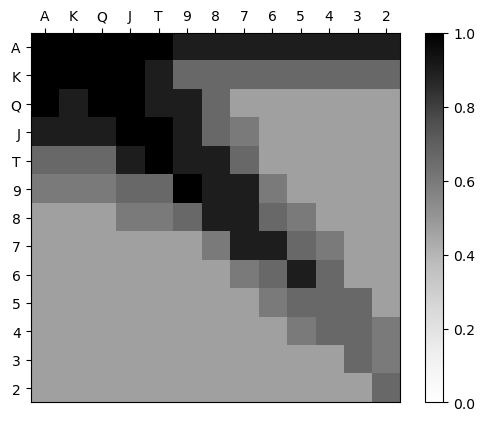
\includegraphics[width=\textwidth/2]{graphics/weights.png}
    \caption{Adjustment matrix example.}
    \label{fig:matrix}
\end{figure}

\subsection{Opponent Ranges}

PokerShark uses the previous ratios to infer the opponent's playing style. Additionally, an adjustment matrix is created for each opponent. The adjustment matrix has an entry for each possible pocket. Each entry represents the probability of the opponent holding that pocket. This matrix is updated following each action the opponent performs based on its playing style.

The adjustment matrix starts with all possible pockets being equally likely to be played by the opponent. After each decision, the opponent makes a set of adjustment factors is chosen based on the observed playing style and applied to the matrix. The calling/raising range of the opponent gets more accurate as the game progresses. Figure \ref{fig:matrixProgression} shows how the adjustment matrix is refined over time. After several rounds, PokerShark will have a basic estimate of the opponent's preferences and playing ranges. 

\begin{figure}[htp]

    \centering
    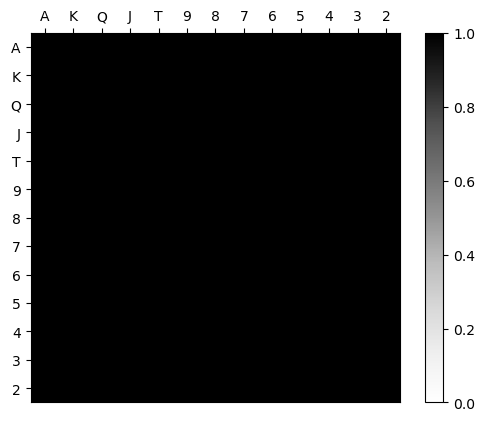
\includegraphics[width=.3\textwidth]{graphics/round_1.png}\hfill
    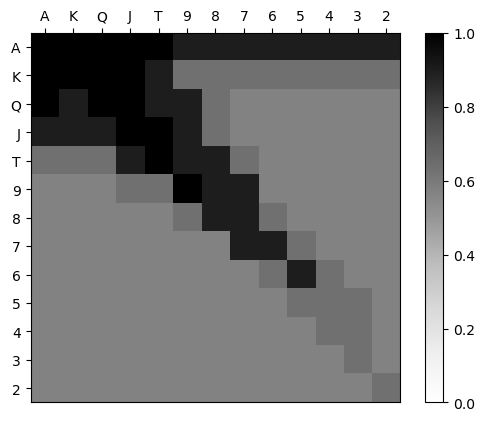
\includegraphics[width=.3\textwidth]{graphics/round_5.png}\hfill
    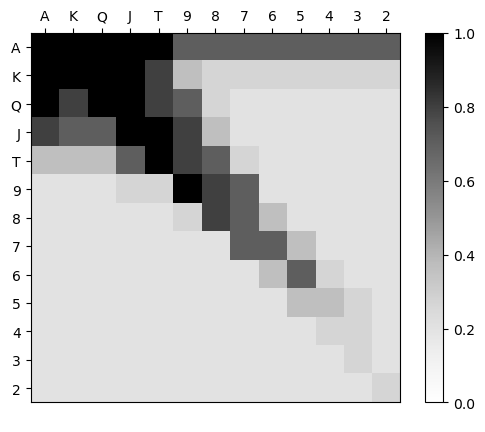
\includegraphics[width=.3\textwidth]{graphics/round_15.png}
    
    \caption{Adjustment matrix progression.}
    \label{fig:matrixProgression}
    
\end{figure}

The opponent's decision-making process is complex and involves many factors, such as position, the opponent's perception of other players, pot size, stack size, and many other factors. Therefore, we can not pretend that having an estimate of the preferred playing ranges is sufficient. However, it is important to understand how PokerShark interprets and utilizes this model to make better decisions, which we will explore in the next sections.

